%%% LaTeX Template: Article/Thesis/etc. with colored headings and special fonts
%%%
%%% Source: http://www.howtotex.com/
%%% Feel free to distribute this template, but please keep to referal to http://www.howtotex.com/ here.
%%% February 2011
%%%
%%% Modified October 2015 by CDM

%%%  Preamble
\documentclass[11pt,letterpaper]{article}
\usepackage[margin=1.0in]{geometry}
\usepackage[T1]{fontenc}
\usepackage[bitstream-charter]{mathdesign}
\usepackage[latin1]{inputenc}					
\usepackage{amsmath}						
\usepackage{xcolor}
\usepackage{cite}
\usepackage{hyphenat}
\usepackage{graphicx}
\usepackage{float}
\usepackage{subfigure}
\usepackage{sectsty}
\usepackage[compact]{titlesec} 
\usepackage[tablegrid]{vhistory}
\allsectionsfont{\color{accentcolor}\scshape\selectfont}

%%% Definitions
\definecolor{accentcolor}{rgb}{0.0,0.0,0.5} 
\newcommand{\teamname}{Team Demeter}
\newcommand{\productname}{Polar FarmBot}
\newcommand{\coursename}{CSE 4316: Senior Design I}
\newcommand{\semester}{Fall 2016}
\newcommand{\docname}{Project Charter}
\newcommand{\department}{Department of Computer Science \& Engineering}
\newcommand{\university}{The University of Texas at Arlington}
\newcommand{\authors}{Arun Kalahasti \\ Bipin Ghimire \\ Saman Shrestha \\ Santosh Pradhan \\ Travis Matthews}

%%% Headers and footers
\usepackage{fancyhdr}
	\pagestyle{fancy}						% Enabling the custom headers/footers
\usepackage{lastpage}	
	% Header (empty)
	\lhead{}
	\chead{}
	\rhead{}
	% Footer
	\lfoot{\footnotesize \teamname \ - \semester}
	\cfoot{}
	\rfoot{\footnotesize page \thepage\ of \pageref{LastPage}}	% "Page 1 of 2"
	\renewcommand{\headrulewidth}{0.0pt}
	\renewcommand{\footrulewidth}{0.4pt}

%%% Change the abstract environment
\usepackage[runin]{abstract}			% runin option for a run-in title
%\setlength\absleftindent{30pt}			% left margin
%\setlength\absrightindent{30pt}		% right margin
\abslabeldelim{\quad}	
\setlength{\abstitleskip}{-10pt}
\renewcommand{\abstractname}{}
\renewcommand{\abstracttextfont}{\color{accentcolor} \small \slshape}	% slanted text

%%% Start of the document
\begin{document}

%%% Cover sheet
{\centering \huge \color{accentcolor} \sc \textbf{\department \\ \university} \par}
\vspace{1 in}
{\centering \huge \color{accentcolor} \sc \textbf{\docname \\ \coursename \\ \semester} \par}
\vspace{0.5 in}
\begin{figure}[h!]
	\centering
   	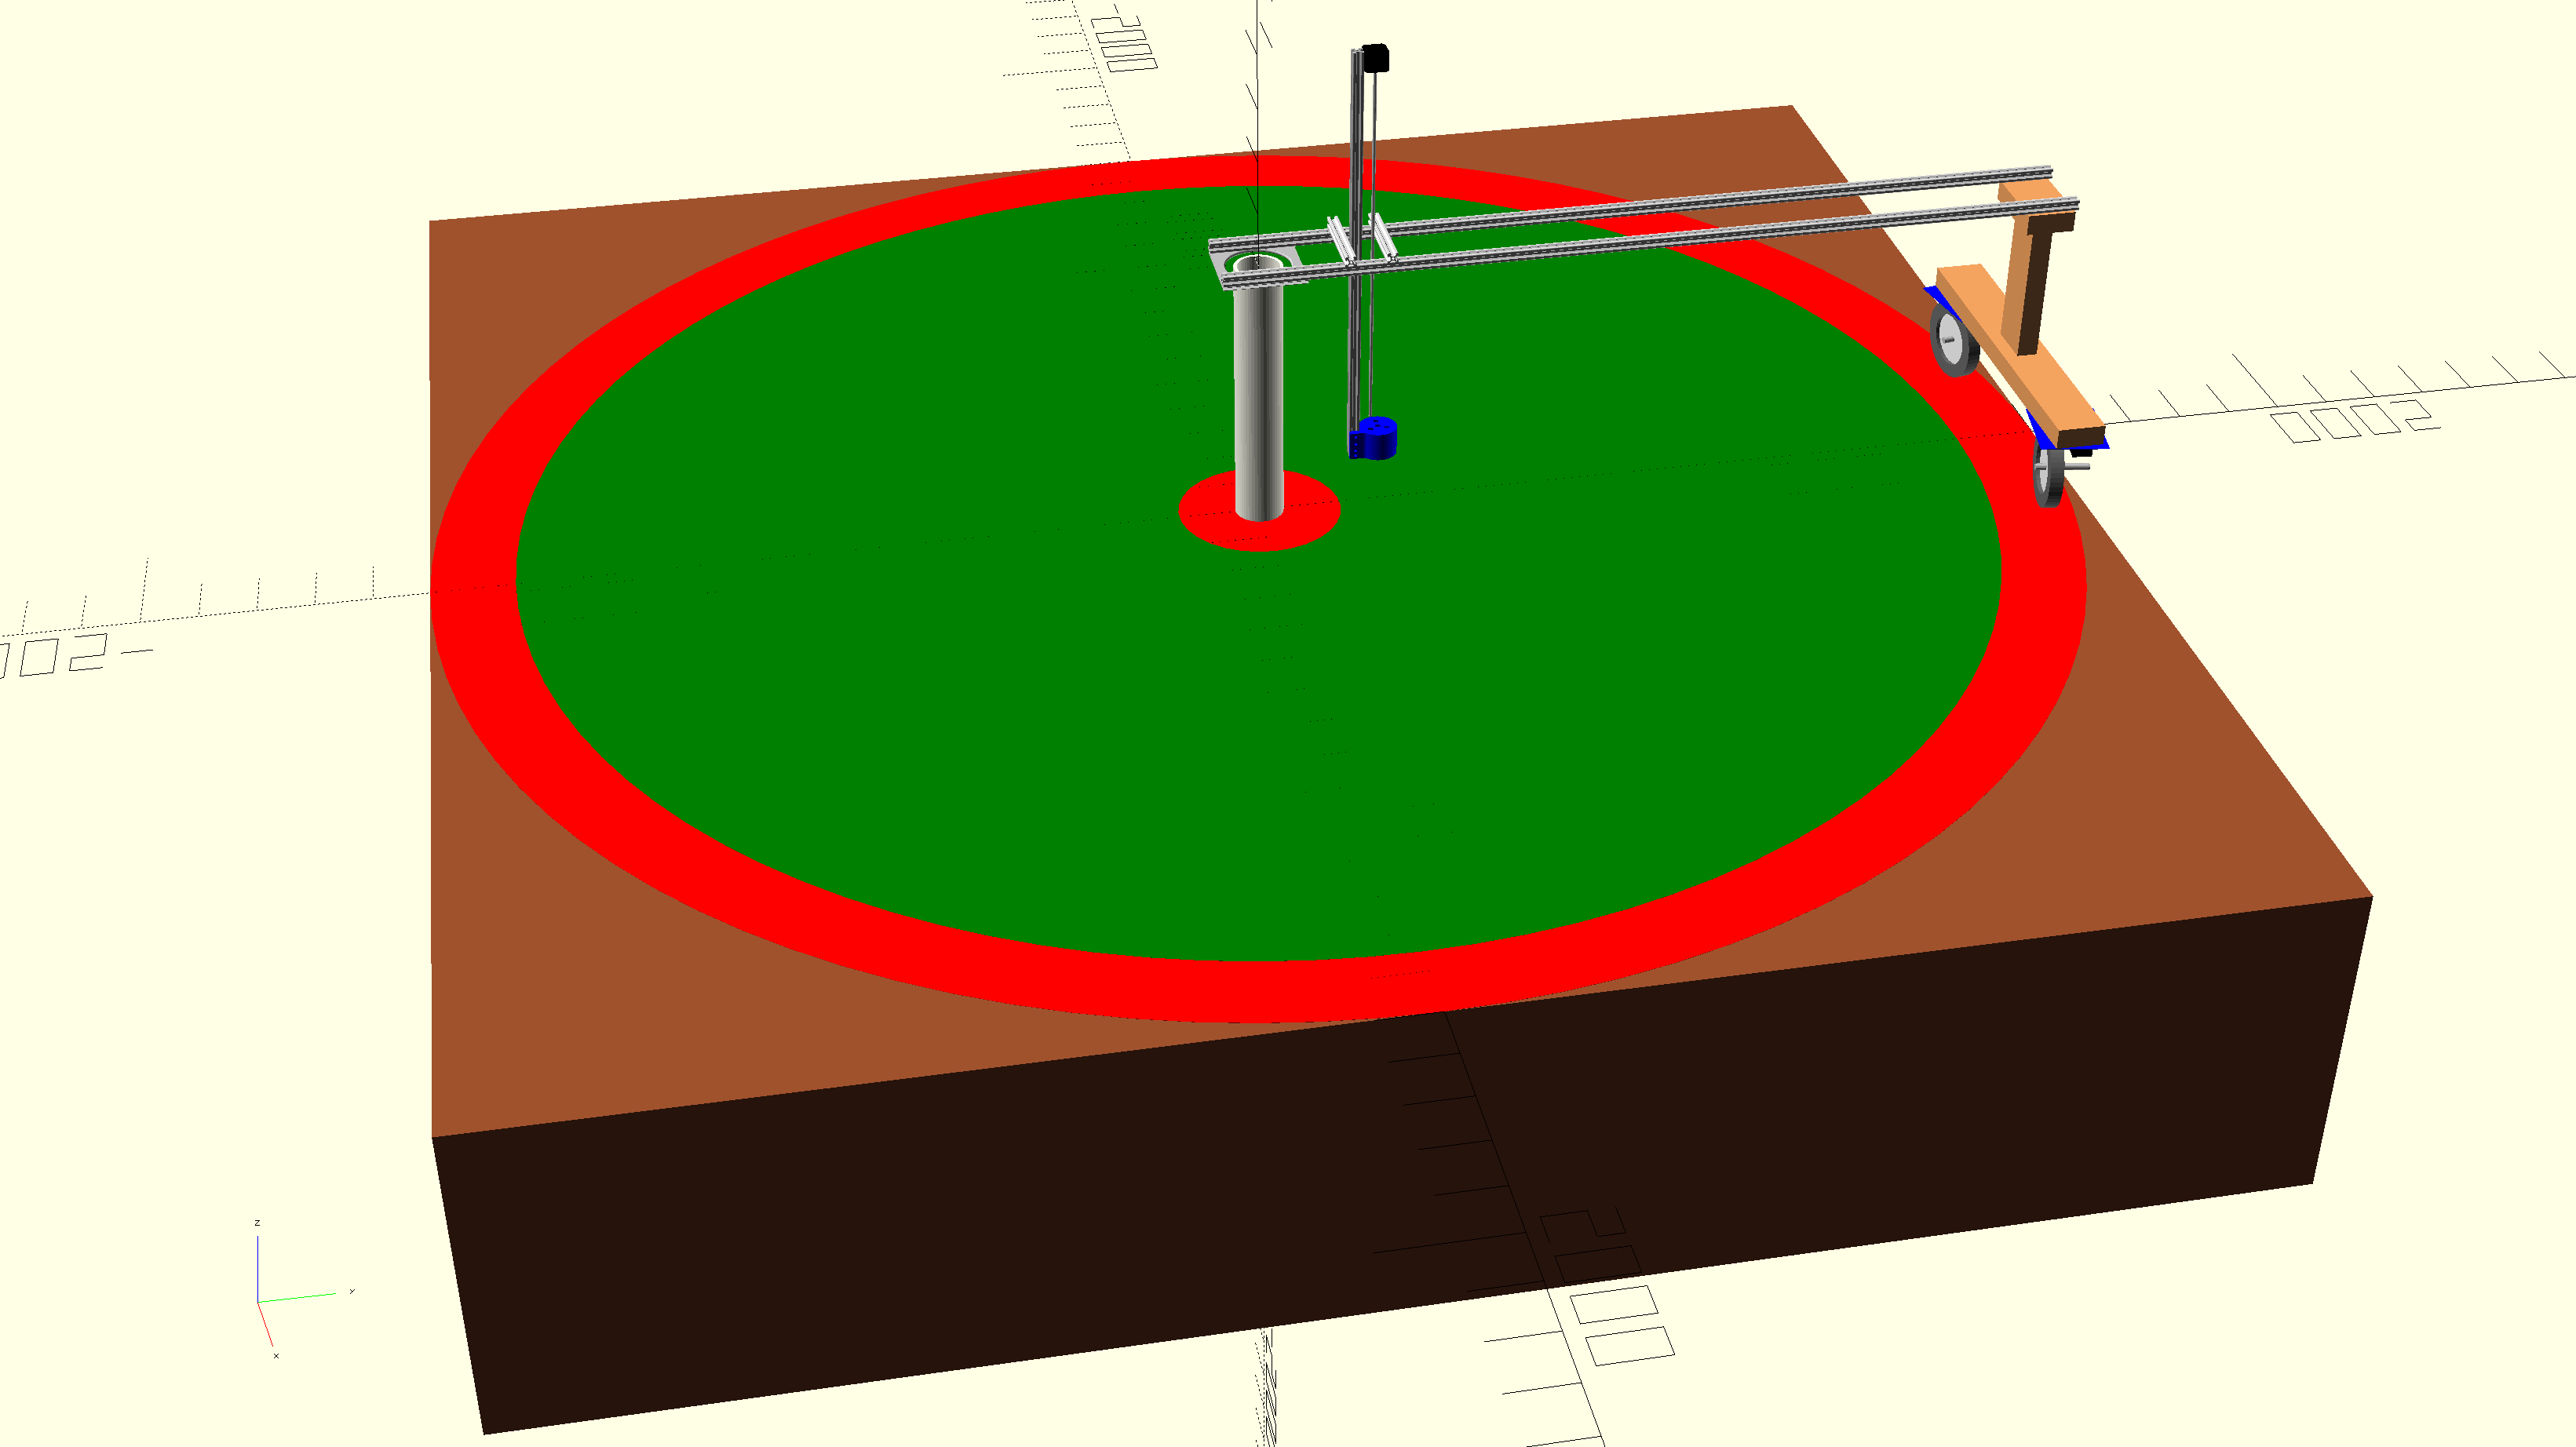
\includegraphics[width=0.60\textwidth]{images/mock-up}
\end{figure}
\vspace{0.5 in}
{\centering \huge \color{accentcolor} \sc \textbf{\teamname \\ \productname} \par}
\vspace{0.5 in}
{\centering \large \sc \textbf{\authors} \par}
\newpage


%\vspace{1 in}
%\centerline{January 13th, 2012}
%\newpage

%%% Revision History
\begin{versionhistory}
  	\vhEntry{0.1}{09.24.2016}{AK}{document creation}
\end{versionhistory}
\newpage

%%% Table of contents
\tableofcontents
\newpage

%%% List of figures and tables (optional)
\listoffigures
%\listoftables
\newpage

%%% Agile project charter sections
\section{Vision}
Farming does not have to be a full time job but in the traditional way of farming a lot of time and space is required. A problem with traditional farming is that the general people who work 8-5 job cannot aside enough time and generally does not have enough space to farm using traditional method. To address those problems, we are building a farming robot called Frambot. It is a small robot which replaces humans to some extent from farming. Farmbot requires a small space as well as a very little attention. Farmbot can be an effective solution.
\section{Mission}
The proposed design is a polar machine which will consist of a tool gantry, an arm which the gantry will ride on, a pivot which the arm will roatate around, and a wheeled extension at the other side of the arm.
The outer perimeter section will be supported by a pair of motorized wheels which will provide angular motion.
The main arm will conist of a pair of rods and a motorized belt. The mobile ganrty will be attached to the belt to adjust the radial distance of the gantry from the central pivot point. 
\section{Success Criteria}
This project will be considered successful if the outcome is able to replicate the core functionalities dislpayed by the FarmBot, namely the ability to plant seeds, water plants, monitor growth, and kill weeds. That goal will require the construction of a polar coordinate robotic platform which is compatiable with the FarmBot tooling system as well as a series of modifications to the FarmBot software backend to allow the system to operate in the new platform envelope.
\newpage

%%% Remaining project charter sections
\section{Background}
This project is an offshoot of a senior design initiative. It was origially proposed as a smart irrigation system which would use low cost wirelessly connected nodes to control water distribution and collect sensor data across a crop field. That initial proposal was rejected by the Product Owner due to insufficient hardware complexity and the FarmBot was recommended as an alternate goal. The design team proposed an alteration of the FarmBot design inspired by center pivot irrigation systems, which was accepted by the Product Owner. We chose to pursue that design because it addresses a very common problem in the modern consumer world: The inability to grow foods at home. Due to tight schedules and the exhausting work many people operate with, it is simply not feasable for them to grow a garden. The FarmBot is designed to allow these individuals to grow crops at home, but requires an initial investment most Americans are not willing or able to commit to. We wish to increase the feasability of automated home gardening and lowering the cost of entry with this alternate design.
\section{Related Work}
Our team is trying to replicate a machine called the FarmBot Genesis but we are trying to make our FarmBot better and cheaper. FarmBot Genesis is the first FarmBot designed and prototyped that helps you grow plants. Genesis is a small scale FarmBot primarily constructed from V-Slot aluminum extrusions and aluminum plates and brackets. Genesis is driven by NEMA 17 stepper motors, an Arduino Mega with a RAMPS shield, and a Raspberry Pi 3 host computer. These electronics were chosen for their great availability, support, and usage in the DIY 3D printer world. Genesis can vary in size from a planting area as little as 1m2 to greater than 50m2, while accommodating a maximum plant height of about 1m. With modifications to some of the structural component sizes and an alternative X-direction drive system, the Genesis concept could likely scale up to a 1000m2 planting area and a maximum plant height greater than 2m. The hardware is designed to be durable, easily assembled and modified with common tools, constructed from largely off-the-shelf components, and manufactured with readily available processes and materials. The FarmBot genesis moves in a XY-axis and it plants seeds, waters them, checks the status of soil and helps destroy weeds.
\section{System Overview}
PolarFarmBot will be a CNC robot that will automate the agricultural process. The robot will pivot around a central pole and have a tool assembly that will moved in and out along the arm of the robot.
PolarFarmBot will plant seeds, water plants, measure soil moisture levels, calculate soil pH levels, and remove weeds.
The robot will connect back to a computer that will have a web interface for users to interact with the robot. From this interface a user will be able to layout a plot, monitor overall plant growth and soil conditions, and see whether or not the plants are ready for harvesting.
To go along with the web interface, there will be a companion application developed for android. This app will have all the same functionality as the web app just on a mobile platform.
PolarFarmBot will have multiple cameras attached to it to allow monitoring progress remotely.


\begin{figure}[h!]
    \centering
    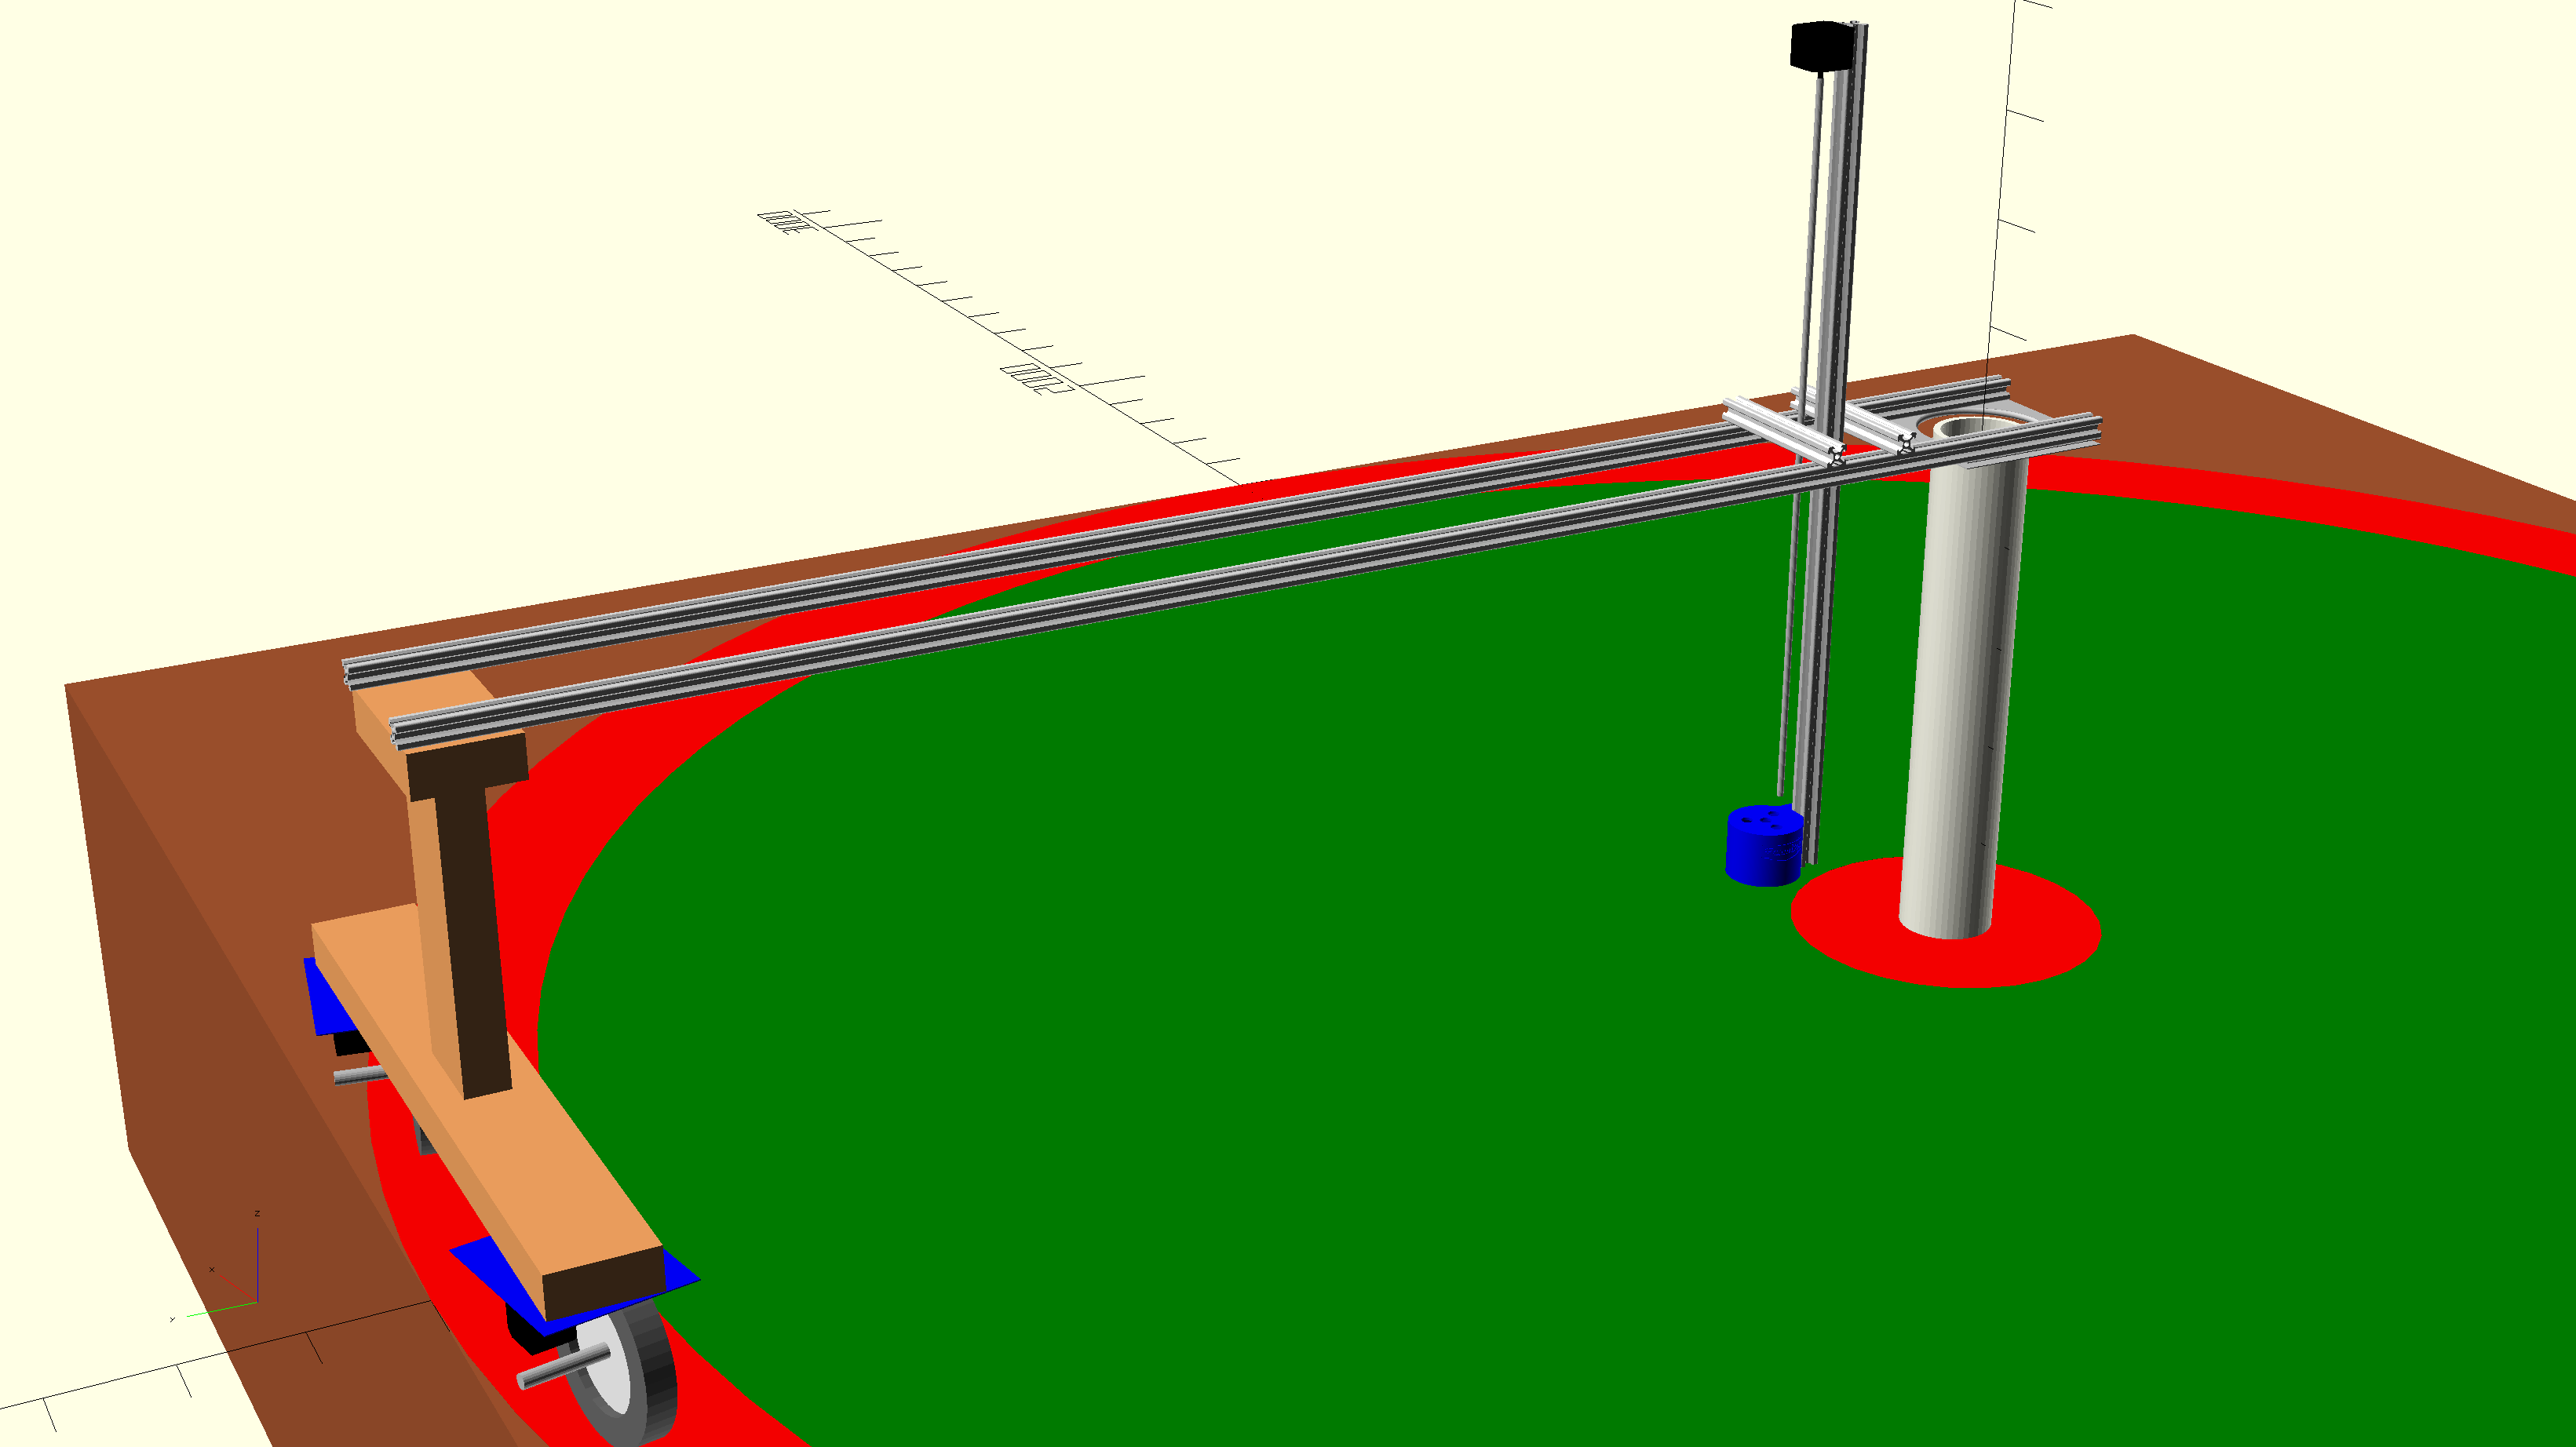
\includegraphics[width=0.75\textwidth]{images/arm-closeup}
    \caption{Deatailed view of mock-up arm design}
\end{figure}
\section{Roles \& Responsibilities}
Arun Kalahasti will lead hardware development, act as Scrum Master for the team, and aid in software design and implementation. As Scrum Master he will be expected to maintain documentation and establish sprint goals. Arun has the most experience in the team with hardware development and implementation, therefore his responibilities as lead harware developer will be to establish and maintain project hardware and physical design. He also has experience with creating systems in many development platforms, incuding Android, Java, C++, C\#, .NET, Javascript, several Javascript frameworks, Arduino, Python, and will therefore contribute to software design and implementation.

Travis Matthews will lead Software Development and aid in hardware design and implementation. Working with Arduino projects and building various electrical circuits, Travis will be able to contribute well to the the hardware design process. Travis also has extensive experience in software development; creating systems in Android, iOS, ASP.NET, Java, C++, C\#, and Python. He will be in charge of building the wireframes for the software systems and come up with how the systems will interface with each other other. Along with managing the software systems, Travis will also be a developer in creating these systems.

Saman Shrestha would work as a general developer. Having a background in computer science he would be better writing codes for the software of the FarmBot. He has worked on various coding platforms and is good in Java, C and python. He would also help in building the bot. He is really interested on the hardware aspect of the project and would help putting the bot together.

Santosh Pradhan will assist in Software Development and also in hardware design and implementation. He has an experience working in java, c, python and database. He will also contribute in building electrical circuits and assembling different hardware parts. Also, he will be researching and helping out to design an efficient and economical robot. 

Bipin Ghimire will help building the software and harware of the project and also assist in research of the project.

\section{Facilities \& Equipment}
The development and prototyping of PolarFarmBot will take place in the Senior Design Lab.
All the hardware design and development will take place in the lab during the Senior Design I semester. We will be using the 3D printers to make housings for the motors and various parts on the robot.
We will also be using common tools such as the drills, screwdrivers, saws, and Allen wrenches from the Senior Design Lab.
Tools that are not available from the lab will be donated or leased from Partsmaster, a company helping out our team in the building of the robot. If there is special heavy machinery that we need that is not available in the Senior Design Lab nor Fab Lab, Partsmaster has said we can use any machinery in their shop.
Upon building the successful prototype, our team will implement a full scale 13' x 13' robot in the backyard of one of our team member's home.

\section{Cost Proposal}
Cost Proposal: We have default 800 budget provided by UT Arlington department sponsorship funds.  Since, our team do not have any company sponsors for the project, we are currently seeking donations from different companies. Once we gather all the parts from donations, we will buy the remaining parts that we need with our default budget.

Preliminary Budget: The basic categories of components for our Farmbot project are Extrusions, Plates, Fasteners and Hardware, Drivetrain, Electronics and Wiring, Tubing, 3D Prints and Miscellaneous. Our team has estimated to spend about \$100 on Drivetrain, \$200 on Electronics and around \$200 on Miscellaneous since it will include the frame we build the robot in. Here, Extrusions are taken care of through the lab . Fasteners and Hardware and Tubing are covered with the donations from two companies namely Danco and Partsmaster. We are going to use our teammate Arun's 3D printer. We are going to 3D print all the required plates for our project.

Current \& Pending Support: So far, with the great work from our team mate Travis, two companies namely Danco and Partsmaster have already made donations of the following items for our projects:


a> 25' Extension Cord

b> 50' of 18 \& 20 Gauge wire

c> Clamps

d> 25' 1/4" inner diameter tubing

e> 4 sets of 1/4" Barbs

f> Cable ties

g> Electrical Tape

h> Wire Strippers

i> Soldering Iron

j> Solder

k> Wet/dry vacuum

l> All the screws we need

m> 16 motion computing le 1600 computers


Also, our team mate Arun has provided us with 3D printers, 1700 mm of aluminium rod and 20mm*20mm t-slot rail.

\section{Documentation \& Reporting}
This section describes our intentions for documentation upkeep and expected deliverables for the duration of the project.

\subsection{Project Charter}
This project charter will detail the target goals desired by the team working to it's completion.

\subsection{Product Backlog}
The product backlog is to maintain a list of what work the team will need to deliver for a fully functional product. We will maintain a product backlog on a Team Foundation Server instance hosted on Visual Studio Online. The backlog will be ordered by the product owner from what is considered most important at the top of the backlog to what is considered least important at the bottom of the backlog.

\subsection{Sprint Planning}
We intend to hold sprint planning sessions after our regularly planned meetings. Team members will propose task, features, and other work for upcoming sprints during these sessions. If a majority of the team agrees to commit to completing a work item, it will be estimated for difficulty and entered into the upcoming sprint.

\subsubsection{Sprint Goal}
The sprint goal will be decided by a team vote. 

\subsubsection{Sprint Backlog}
The sprint backlog will be decided by the product owner. The product owner will select the most important items from the top of the product backlog.

\subsubsection{Task Breakdown}
Tasks will assigned to team members who volunteer for them. Remaining tasks will be assigned by 

\subsection{Sprint Burndown Charts}
A sprint burndown chart will be generated by the Scrum Master at the end of every sprint cycle. 

\subsection{Sprint Retrospective}
A sprint retrospective will be held at the first team meeting after the ending of each sprint. 

\subsection{Individual Status Reports}
Individual status reports will be made during the regularly held team meetings. Any exceptionally important information should be posted to the team text communications channels.

\subsection{Engineering Notebooks}
The team members will maintain individual engineering notebooks which will be peer reviewed and signed by other members of the team.

\subsection{Closeout Materials}
At the conclusion of this project we will deliver a functional prototype with a documented assembly guide to replicate the project and all software needed to operate the prototype. This software will be delivered with instructional guides to help with installation. 

\subsubsection{System Prototype}
The system will be prototyped in two stages. The first phase is a pure hardware design phase, during which a small scale unit will be constructed.This small scale unit will be used to develop control firmware and finalize the design of the primary components, but will be constructed in limited space. During the second development stage a second prototype will be created which will utilize all the mechanical designs developed during the first stage, but without space limitations. 

\subsubsection{Project Poster}
We will design and produce a poster to help explain the problem we are trying to address, the solution we are proposing, differences between our project and the FarmBot project, and finally demonstrate our design solution.

\subsubsection{Web Page}
We will make a simple interactive web page which will demonstrate the project and link to further documentation. The web page will also credit all our sponsors.

\subsubsection{Demo Video}
A full system operation video will be made a link to that video will be available on the product web page.

\subsubsection{Source Code}
The source code for the project will be made available on a public git based repo.

\subsubsection{Source Code Documentation}
The source code will be documented with Doxygen and made available with the source code.

\subsubsection{Hardware Schematics}
Hardware scematics will be posted with the source code.

\subsubsection{CAD files}
CAD files will be made with OpenSCAD and will be part of the source code.

\subsubsection{Installation Scripts}
The project deliverables which are designed to be deployed by users will have installation scripts. Documentation will be delivered with the instillation scripts to guide users through their use.

\subsubsection{User Manual}
The user manual will be created on a wiki style site. This will allow maintenance by dedicated users after the project is delivered.
\newpage

%%% References
\bibliographystyle{plain}
\bibliographystyle{reference/IEEEtran_custom}
\bibliography{reference/refs}{}

\end{document}